\documentclass[11pt,a4paper]{article}

%%%%%%%%%%%%%%%%%%%%%%%%% packages %%%%%%%%%%%%%%%%%%%%%%%%

%\documentclass{aimsessay}
\usepackage[utf8]{inputenc}
\usepackage[english]{babel}

%Import the natbib package and sets a bibliography  and citation styles
\usepackage{natbib}
\usepackage{amsmath}
\usepackage{amssymb}
%\usepackage{natbib}
\usepackage{amsthm}
\usepackage{amsfonts}
\usepackage{graphicx}
\usepackage{siunitx}
%\usepackage[utf8]{inputenc}
%\usepackage[english]{babel}
\usepackage[all]{xy}
\usepackage{float}
\usepackage{tikz}
\usepackage{verbatim}
\usepackage[left=2cm,right=2cm,top=2cm,bottom=2cm]{geometry}
\usepackage{hyperref}
\hypersetup{
	colorlinks=false,
	linkcolor=blue,
	filecolor=magenta,      
	urlcolor=cyan,
	pdftitle={Overleaf Example},
	pdfpagemode=FullScreen,
}
\usepackage{caption}
\usepackage{subcaption}
\usepackage{psfrag}

\usepackage{url} 
%\bibliographystyle{abbrvnat}
\usepackage{booktabs}  
\usepackage[T1]{fontenc}    % use 8-bit T1 fonts
%\usepackage[nottoc]{tocbibind}

\usepackage{url} 

\newcommand{\donna}[1]{{\color{red}{#1}}}   
\newcommand{\ignore}[1]{}

%%%%%%%%%%%%%%%%%%%%% students data %%%%%%%%%%%%%%%%%%%%%%%%
\newcommand{\student}{Brian KYANJO }
\newcommand{\course}{Dr. Jodi Mead, Michal Kopera, and Dylan Mikesell}
\newcommand{\assignment}{ Prof. Donna Calhoun}


%%%%%%%%%%%%%%  Shortcut for usual set of numbers  %%%%%%%%%%%

\newcommand{\N}{\mathbb{N}}
\newcommand{\Z}{\mathbb{Z}}
\newcommand{\Q}{\mathbb{Q}}
\newcommand{\R}{\mathbb{R}}
\newcommand{\C}{\mathbb{C}}

%%%%%%%%%%%%%%%%%%%%%%%%%%%%%%%%%%%%%%%%%%%%%%%%%%%%%%%555
\begin{document}
	
	%%%%%%%%%%%%%%%%%%%%%%% title page %%%%%%%%%%%%%%%%%%%%%%%%%%
	\thispagestyle{empty}
	\begin{center}
		\textbf{A Riemann Solver for Wet/Dry Interfaces in Finite Volume Schemes\\[0.5cm]
			Synthesis Paper}
		\vspace{.2cm}
	\end{center}
	
	%%%%%%%%%%%%%%%%%%%%% assignment information %%%%%%%%%%%%%%%%
	
	\begin{center}
		\rule{17cm}{0.2cm}\\[0.3cm]
	\end{center}	
	
	\noindent	Name: \student \hfill Supervisor: \assignment\\[0.1cm]
	Committee: \course \hfill Date: \today\\
	\rule{17cm}{0.05cm}
	\vspace{.2cm}
	
	\section{Introduction}
	

%	\donna{	
				A tsunami is a series of energetic water waves generated due to the displacement of large volumes of water by different mechanisms such as earthquakes, volcanic eruptions, underwater landslides, and local landslides along the coast. According to the recent tragic events in December 2004 in Indonesia and  South Africa, tsunamis may be extremely catastrophic: they can lead to the loss of human lives and destroy buildings and roads. Typically, they cause devastative damages to infrastructures. Deep knowledge of tsunamis is required to provide early warning messages to the regions that may be affected, carry out necessary evacuations, and also anticipate the highest run-ups and run-downs \cite{sanchez2016uncertainty}.
				
				Most numerical tsunami models rely on solving Riemann problems which can robustly track wetting and drying interfaces to model run-up on beaches and inundation into harbors and communities along the affected coastlines.  Various approaches have been taken to handle these wetting and drying states. For instance, \citet{ge:2011} used Godunov-type finite volume methods to model inundation by allowing cells to shift from dry to wet near refinement boundaries dynamically. 
				
				
			Furthermore, \citet{barzgaran2019numerical}  used an augumented Riemann solver coupled with a second-order finite volume method to simulate bedload sediment transport. Results proved that this efficient method is capable of modeling wet/dry interfaces and investigated flow regimes. In addition, the technique employed wave decomposition and the flux-wave formula, which made bed variations vary as four waves propagated from each cell interface.
			
			
%}


	\section{Shallow water equations for tsunami modeling}
	%\donna{	
	Shallow water models have been frequently used to handle the propagation of tsunami waves in the ocean see for instance \citet{dutykh2007water,le-ge-be:2011,dias2007dynamics}. The SWE assumption is applicable as the average ocean depth is very shallow compared to the tsunami's wavelength. In addition, the amplitude of tsunami is minimal offshore, typically less than 1m, to justify the smallness \donna{shallowness?} assumption. 
	
		The shallow water wave equations (SWE) are a system of hyperbolic PDEs governing the flow below a pressure surface in a fluid. They arise from the Navier-Stokes equations.  In one dimension, the SWE  can be used to model a fluid in a channel of unit width, taking the vertical velocity negligible and horizontal velocity roughly constant throughout any cross-section of the channel \cite{ge:2008}.  
		
		Consider small-amplitude waves in a one-dimensional fluid channel that is shallow relative to its wavelength. The conservation of momentum equation is written in terms of pressure, $p(x,t) = \frac{1}{2}\rho gh^{2}$, and the height field $h(x,t)$ ($m$), which breaks down into system \eqref{p2}.
	\begin{equation}
		\begin{aligned}
			h_{t} + (uh)_x &= 0 \\
			(hu)_t + \left(hu^{2} + \frac{1}{2}\rho gh^{2} \right)_x & = 0 
		\end{aligned}
		\label{p2}
	\end{equation}	
	where $hu$ measures the flow rate of water past a point,  $\rho$ (\si{\kg/\m^3}) is the constant density of the in-compressible fluid, and $u(x,t)$ ($m/s$) is the horizontal velocity \cite{chaabelasri1849simple} \donna{Is this really where someone would go to learn more about shallow water wave equations?  Toro or LeVeque would be better references.}.  We will set $\rho = 1$ here.
	
	A simple set of initial conditions is a single discontinuity at the middle of the channel.  In this case, we set $h$ and $hu$ equal to constants on either side of the medium.  This problem is a classic Riemann Problem, and the SWE has an exact solution.  We assume the discontinuity is at $x = 0$; its associated Riemann problem is the initial value problem initial conditions of:
		\begin{eqnarray}
		q(x,0)& =& \begin{cases}
			q_{l}, & \text{if \, $x \le 0,$}\\
			q_{r},& \text{if \, $x > 0,$}\\
			
		\end{cases}  
		\label{rp1}     
	\end{eqnarray}
where $q_{l}$ and $q_{r}$ are two piece-wise constant states separated by a discontinuity \cite{ba-le-mi-ro:2003}. 

	The variation of $h$ and $hu$ on either side of the discontinuity leads the waves in the Riemann problem to move at different speeds creating discontinuities (shocks) or changing regions (rarefactions)\cite{leveque2002finite}.  At $x = 0$ and $t = 0$,   the discontinuity is located between the left and right state, so the solution at the left ($q_{l}$) and right($q_{r}$) states are given by: 
	\begin{equation}
		q_{l} = \begin{bmatrix}
			h_{l} \\( hu)_{l}
		\end{bmatrix}  \quad \text{and} \quad q_{r} = \begin{bmatrix}
			h_{r} \\( hu)_{r}
		\end{bmatrix} 
		\label{ic}
	\end{equation}
	As $t$ increases, four distinct regions are created, separated by characteristics. The middle state called the intermediate state($q_{m}$) is generated.  The determination of this state characterizes the Riemann problem and how it connects to other states via waves in each respective characteristic family\cite{ba-le-mi-ro:2003}.  This can only hold if the connection wave speeds satisfy the Lax entropy condition. Figure \ref{fig:x-tplane} shows a wave combination of a centered rarefaction and shock wave from the first and second characteristic family, respectively.
	
	\begin{figure}[H]
		\centering
		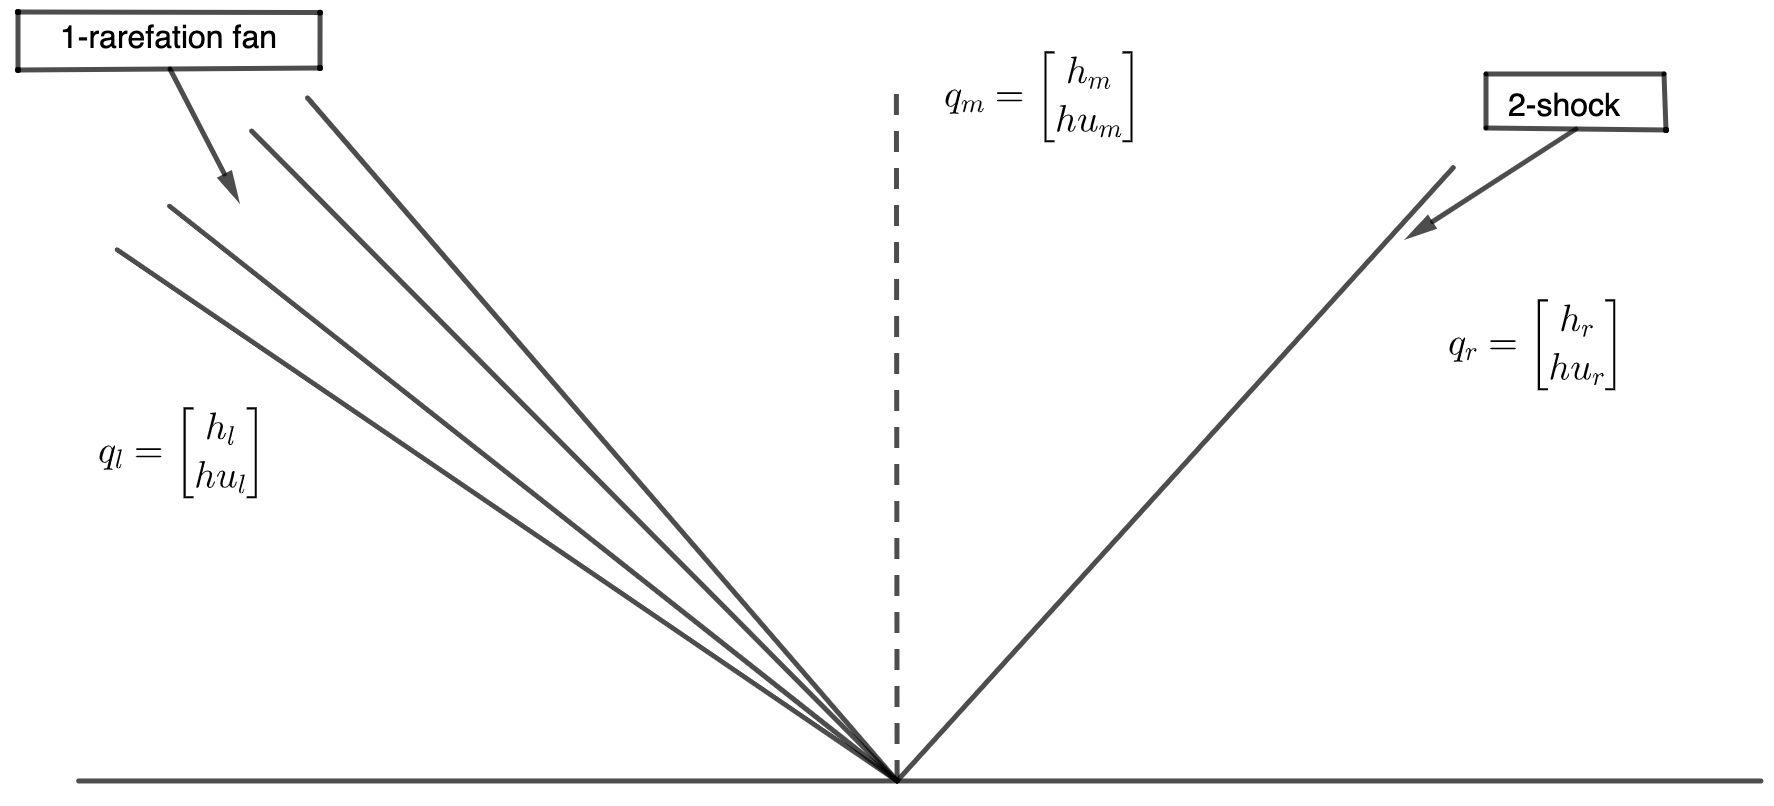
\includegraphics[width=0.5\linewidth]{images/geo1}
		\caption{ x-t plane showing the connection of states, 1-rarefaction fan, and the 2-shock.}
		\label{fig:x-tplane}
	\end{figure}

	\donna{Add x-axis and y-axis labels to figure.}
	
	The intermediate state is obtained by solving the Riemann problem using the exact or approximate method. Approximate methods are widely used due to their cheap computational cost compared to the exact solvers\cite{bu-ku-we-da:2009}.
	
	\donna{Include a three or four plots showing initial conditions, and the evolution of a shock and rarefaction. }

	\subsection{Exact Riemann Solver for two-shock SWE}
The states in \ref{fig:x-tplane} are separated by either {\em shocks} or {\em rarefactions}. General left, and right states will be connected by a combination of the two (either two shocks, two rarefactions, or one of each).  We describe how to determine if a shock connects two states.  We refer the reader to \cite{leveque2002finite} for other cases. 

We can achieve an exact solution to the Riemann Problem for the SWE as follows. 
The shock speed, $s(t)$,  from the shock wave as the solution emerges is determined from the Rankine-Hugoniot jump condition given by equation \eqref{e1}  which must be satisfied across any shock wave.  If $q_l$ and $q_r$ are connected by a shock, the Rankine Hugoniot conditions will be satisfied\cite{ma-ah-be-ca-ge-ha-ke-le-le:2016}. 
	\begin{equation}
		\begin{aligned}
			s_1(q_{m} - q_{l}) & = f(q_{m}) - f(q_{l}) \\
			s_2(q_{r} - q_{m}) & = f(q_{r}) - f(q_{m})
		\end{aligned}
		\label{e1}
	\end{equation}
	By applying condition  \eqref{e1} to shallow water equations \eqref{p2}  creates a system of four equations that must be satisfied simultaneously. 
	
	Not all left and right states can be connected by a shock wave.  In this case, we connect states by a rarefaction wave. See Figure (\ref{hor1})  for illustration of the evolution of a Riemann problem for the all shock case \ref{allshock} and for a case in which the right going wave is a shock \ref{2shock}, all rarefaction case \ref{allrare}, and the left going wave is a rarefaction \ref{1rare}.
	
\begin{figure}[H]%
	\centering
	\subfloat[]{%
		\label{allshock}  %
		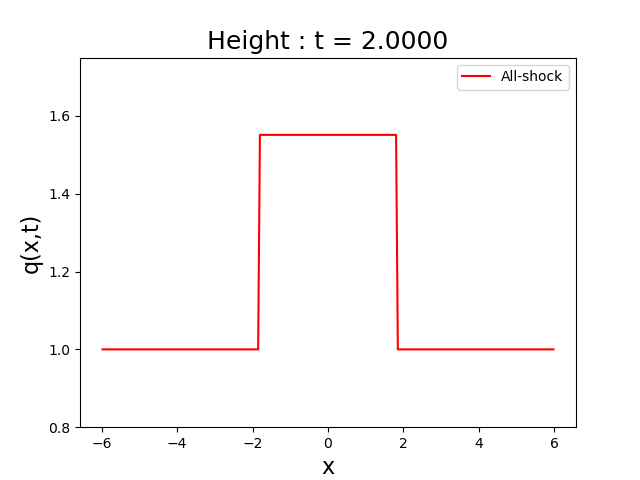
\includegraphics[width=0.4\textwidth, height=5cm]{images/allshock}}
	\quad
	\subfloat[]{%
		\label{2shock}  %
		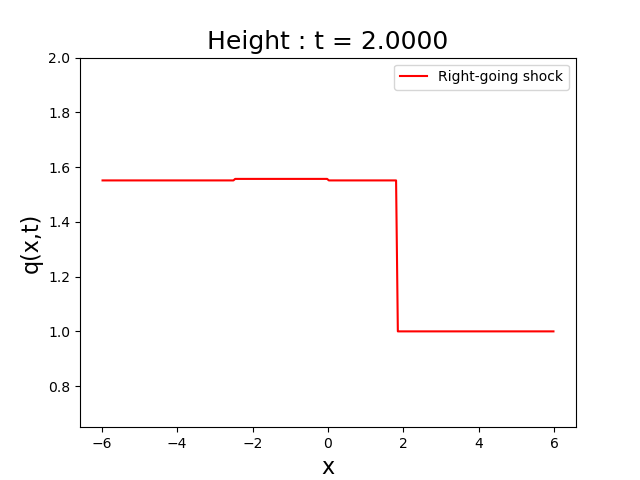
\includegraphics[width=0.4\textwidth, height=5cm]{images/2shock}}%
	
	\subfloat[]{%
		\label{allrare}  %
		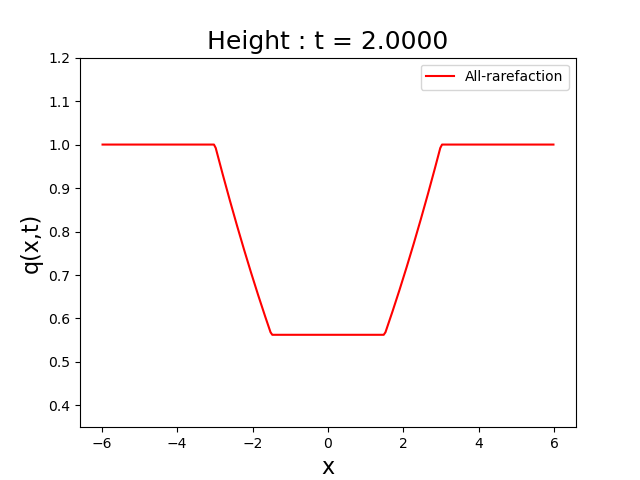
\includegraphics[width=0.4\textwidth, height=5cm]{images/allrare}}
	\quad
	\subfloat[]{%
		\label{1rare} %
		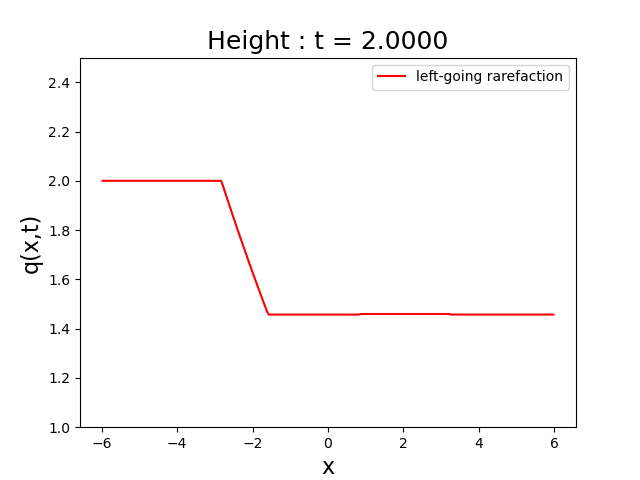
\includegraphics[width=0.4\textwidth, height=5cm]{images/1rare}}%
	\caption{Spatial evolution of the height field for the {\em all-shock case},  {\em right-going shock case}, {\em all-rarefaction case},  and {\em left-going rarefaction case} simulated  at its final time step ($t=2~seconds$) are depicted by (a), (b), (c), and (d) respectively.}
	\label{hor1}
\end{figure}

	\subsection{Finite volume discretization}
Finite volume discretizations are widely used in tsunami modeling since they are: well suited for inundation regimes, robust in the presence of drying regions, well-balanced, and can capture the inundating shoreline and run-up features, see for instance \citet{ge:2008,ge:2011,george2006finite,be-ge-le-ma:2011,bi2014finite,leveque2002finite,ba-le-mi-ro:2003}. The finite volume schemes rely on exact or approximate solutions to the Riemann problem described above.

Consider a one dimensional (1D) conservation law  (equation \eqref{fvm0}),  where $q$ is the measure of conserved quantity density and $f(q)$ is a flux function

	\begin{equation}
		q_{t}(x,t) + f(q(x,t))_{x} = 0.
		\label{fvm0}
	\end{equation}	
	In finite volume methods (FVM), the domain is broken down into grid cells. Consider $C_{i} = (x_{i-\frac{1}{2}},x_{i+\frac{1}{2}})$ to be the $i^{th}$ grid cell, the average value over the $i^{th}$ interval at time $t^{n}$ is numerically approximated by $Q_{i}^{n}$ in equation \eqref{wpa0}.
	
	\begin{equation}
		Q_{i}^{n} \approx \dfrac{1}{\Delta x} \int_{C_{i}}q(x,t^{n})dx
		\label{wpa0}
	\end{equation}
	where $\Delta t = (t^{n+1} - t^{n})$ and  $\Delta x = (x_{i+\frac{1}{2}} - x_{i-\frac{1}{2}})$ is the cell length. A discontinuity in $q$ violates the PDE in the classical sense and only holds for the integral conservation law (fundamental equation \eqref{fvm1}) \cite{leveque2002finite}. Therefore at grid points near discontinuities where PDEs don't hold, all classical finite difference methods breakdown, resorting to FVM which are based on \eqref{fvm1}. 	
	\begin{equation}
		\frac{d}{dt} \int_{c_{i}} q(x,t)dx = f(q(x_{i-\frac{1}{2}},t)) -  f(q(x_{i+\frac{1}{2}},t))
		\label{fvm1}
	\end{equation}	
	The approximate  total integral of $q$ over each grid cell is evaluated and updated at every time step by the grid cell edge fluxes. The determined numerical flux functions evaluate the  cell averages over a certain volume, which are used to approximate the solutions within the cells, using equation \eqref{cellupdate} \cite{le-ge-be:2011}.
	
	\begin{equation}
		Q_{i}^{n+1} = Q_{i}^{n} - \frac{\Delta t}{\Delta x} (F_{i+\frac{1}{2}}^{n} - F_{i-\frac{1}{2}}^{n})
		\label{cellupdate}
	\end{equation}	
	where $F_{i+\frac{1}{2}}^{n} $ is the average flux approximation along $x=x_{i-\frac{1}{2}}$.
	The Riemann problem is a fundamental tool in the evolution of FVM. Taking two neighbouring grid cells: $Q_{i-1} = q_{L}$ and $Q_{i} = q_{R}$ to be cell averages, this information is used by the exact Riemann solver to compute numerical fluxes ( $F_{i-\frac{1}{2}}^{n} = \mathcal{F}(Q_{i-1} , Q_{i} )$) \donna{this returns the middle state.  The flux $f(q)$ is then evaluated at this middle state}, that are used to update the cell average at each time step. Then equation \eqref{cellupdate} becomes:
	
	\begin{equation}
		Q_{i}^{n+1} = Q_{i}^{n} - \frac{\Delta t}{\Delta x} \left[ \mathcal{F}(Q_{i} , Q_{i+1} ) - \mathcal{F}(Q_{i-1} , Q_{i} ) \right]
		\label{cellupdat}
	\end{equation}
	where $\mathcal{F}$ is the  numerical flux function $F_{i-\frac{1}{2}}^{n}$ at $q_l = Q_{i-1}$  and $q_r = Q_{i}$.
	

Figures.~\ref{fig:exap} and \ref{fig:exapp}, depicts the first and second-order correction of the approximate solution (flux base wave decomposition (blue)) \cite{ba-le-mi-ro:2003} and the exact Riemann solution(red) for the dam break problem height field simulated at the final time with limiters. Fig.~\ref{fig:exap}  shows that the first-order approximate solution does not coincide with the exact solution at region edges. However, the second order approximate solution \ref{fig:exapp}  fits the exact solution accurately; hence this validates the exact and numerical solutions.
	\begin{figure}[H]
		\begin{subfigure}[b]{0.5\textwidth}
			\centering
			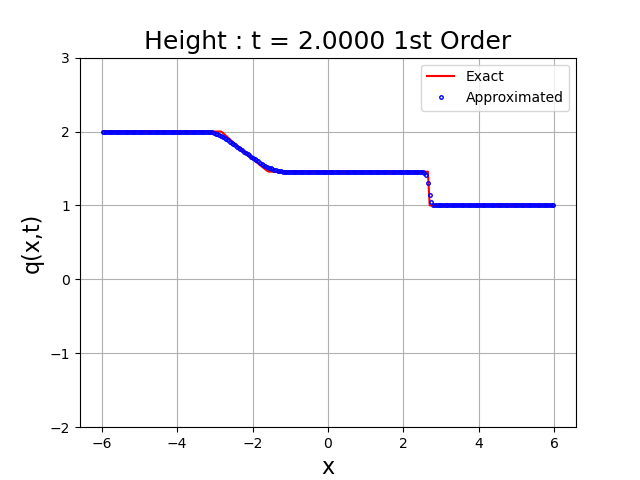
\includegraphics[width=1.0\linewidth]{images/exap}
			\caption{}
			\label{fig:exap}
		\end{subfigure}
		%
		\begin{subfigure}[b]{0.5\textwidth}
			\centering
			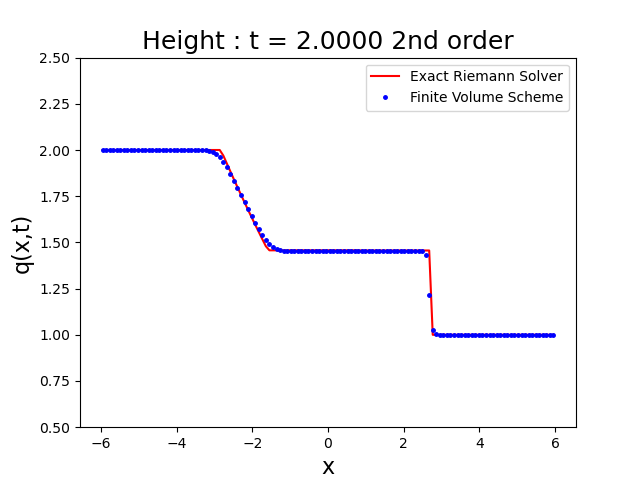
\includegraphics[width=1.0\linewidth]{images/exapp}
			\caption{}
			\label{fig:exapp}
		\end{subfigure}
		\caption{(a) and (b) respectively show height field at the final time step for both first and second order correction with limiters for the exact and approximate solutions. }
	\end{figure}
	\donna{Remove excess white space in figures below y=0.}

	\subsection{Finite schemes in quasi-linear form}
	\donna{Be careful with references here. }
	The general conservation law in \eqref{fvm0} can also be written in {\em quasi-linear form}
as
\begin{equation}
	q_{t} + f'(q)q_{x} = 0
	\label{wpa3}
\end{equation}
where  $f'(q) \in \mathbb{R}^{m\times m}$  flux Jacobian matrix \cite{be-ge-le-ma:2011}.  Consider a Riemann problem for the system  \eqref{wpa3} with initial data 

\begin{equation}
	q(x,t^n)  = \begin{cases}
		Q_{i-1}^{n}  & \text{if} \quad  x < x_{i-\frac{1}{2}}\\
		Q_{i}^{n} & \text{if} \quad x > x_{i-\frac{1}{2}}\\
	\end{cases}    
	\label{w4}   
\end{equation}
The initial data (equation \eqref{w4}), is used by the exact Riemann solver to generate an intermediate state ($q_m = (h_m, hu_m)^T$), which is used to evaluate the eigenvalues ($\lambda_{i-1/2}$) and eigenvectors ($r_{i-1/2}$) at $x = x_{i-\frac{1}{2}}$. The $p^{th}$ wave at interface $i-1/2$ is given by $\mathcal W^p_{i-1/2} \equiv \alpha_{i-\frac{1}{2}} r^p_{i-\frac{1}{2}}$ with speeds $s^p_{i-1/2} = \lambda^p_{i-1/2}$ \cite{leveque2002finite}. where $ \alpha_{i-\frac{1}{2}}$ depicts the coefficients of the the eigenvectors.  Waves and speeds are obtained as an eigenvector decomposition of the jump in $Q_i$ at the interface $i-\frac{1}{2}$.  This decomposition takes the form

\begin{equation}
	Q_{i} -  Q_{i-1} = \sum_{p=1}^{m}  \alpha_{i-\frac{1}{2}} r_{i-\frac{1}{2}} \equiv \sum_{p=1}^{m} \mathcal{W}_{i-\frac{1}{2}}^{p}
	\label{wpa19}
\end{equation}
The wave speed $s_{i-\frac{1}{2}}^{p}$ associated with the vector $r_{i-\frac{1}{2}}^{p}$, are preselected basing on the characteristic structure of the initial Riemann data  \cite{ge:2008}. Therefore the fluctuations $\mathcal{A^{+}}\Delta Q_{i-\frac{1}{2}}^{n}$  and $\mathcal{A^{-}}\Delta Q_{i-\frac{1}{2}}^{n} $ are defined by equations \eqref{f0} and \eqref{f1}:

\begin{eqnarray}
	\mathcal{A^{-}}\Delta Q_{i-\frac{1}{2}}^{n} = \sum_{\{ p:s_{i-\frac{1}{2}}^{p}<0\}} s_{i-\frac{1}{2}}^{p} \mathcal{W}_{i-\frac{1}{2}}^{p}
	\label{f0}\\
	\mathcal{A^{+}}\Delta Q_{i-\frac{1}{2}}^{n} =\sum_{\{ p:s_{i-\frac{1}{2}}^{p}>0\}} s_{i-\frac{1}{2}}^{p} \mathcal{W}_{i-\frac{1}{2}}^{p}
	\label{f1}
\end{eqnarray}

	The second order accuracy is obtained by taking the correction terms into account as shown described in equation \eqref{wpa2} \cite{barzgaran2019numerical}

\begin{equation}
	Q_{i}^{n+1} =  Q_{i}^{n} - \frac{\Delta t}{\Delta x}(\mathcal{A^{+}}\Delta 	Q_{i-\frac{1}{2}}^{n} + \mathcal{A^{-}}Q_{i+\frac{1}{2}}^{n}) -  \frac{\Delta t}{\Delta x} (\tilde{F}_{i+\frac{1}{2}}^{n} - \tilde{F}_{i-\frac{1}{2}}^{n} )
	\label{wpa2}
\end{equation}
where $\tilde{F}_{i-\frac{1}{2}}^{n} $ are second order correction terms determined by the waves and speeds in the Riemann problems after approximating the average flux along  $x = x_{i - \frac{1}{2}}$:

\begin{equation}
	\tilde{F}_{i-\frac{1}{2}}^{n} = \frac{1}{2} \sum_{p=1}^{m}  |s_{i- \frac{1}{2}}^{p}| \left( 1 - \frac{\Delta t}{\Delta x} |s_{i- \frac{1}{2}}^{p}|\right) \tilde{\mathcal{W}}_{i-\frac{1}{2}}^{p} 
	\label{wpa13}
\end{equation}
Here $\tilde{\mathcal{W}}_{i-\frac{1}{2}}^{p} $ depicts a limited version of the wave $\mathcal{W}_{i-\frac{1}{2}}^{p} $, which is obtained after a comparison between $\mathcal{W}_{i-\frac{1}{2}}^{p} $ and $\mathcal{W}_{i-\frac{3}{2}}^{p} $ when $s^{p} >0$ \cite{ba-le-mi-ro:2003}.\\
	
	\subsection{MUSCL approach}
	\donna{Either you talk about general MUSCL schemes or you move this to a section on wetting and drying. }
	
	\subsection{Bathymetry}
	The second challenge in modeling tsunamis is in proper treatment of the bathymetry, or variable ocean bottom. 
	Equation \eqref{p2}, can be extended to balance equations by introducing a bathymetric source term as shown in 

		\begin{equation}
		\begin{aligned}
			h_{t} + (uh)_x &= 0 \\
			(hu)_t + \left(hu^{2} + \frac{1}{2}gh^{2} \right)_x =& -ghB^{\prime}(x).
			\label{bst}
		\end{aligned}
	\end{equation}


	General source terms are typically handled in an operator split approach.  However, for tsunami modeling, this can lead to oscillations in steady state solutions.  A better approach is to discretise the source term to generate values $-gh_{i-\frac{1}{2}}B^{\prime}(x_{i-\frac{1}{2}})$ at  cell interfaces  $x = x_{i-\frac{1}{2}}$. This approach is very useful, because the discrepancy caused due to the failure of the flux gradient to counterbalance the source term in a near steady state solution is decomposed into propagating waves  making the approach more robust than the quasi-steady WPA \donna{what is WPA?}.  This source term balancing approach is described in \cite{ba-le-mi-ro:2003,chaabelasri1849simple.}
	where $B(x)$ represents bottom elevation. \\
	\donna{Bathymetry is handled in an operator split appraoch.}
,
	\donna{Emphasize importance of "well-balanced schemes";  Reference paper by Bale et al.;}


\section{Beach run-up and inundation}

	With a basic understanding of the role that a Riemann solver plays in solving the shallow water wave equations, and the basic finite volume discretization approach, we will describe several approaches to handling wetting and drying.  

	\donna{Describe why we want to modeling the wetting and drying front (beach runup; inundation).   Explain what the Riemann solution looks like (use your last section);  explain what can go wrong (negative height values from \ref{cellupdat}}

	\donna{Describe approaches to handling the wetting and drying front - refer to papers. Can we just set $h = \epsilon$ whenever $h < 0$?}

	\subsection{Riemann Problem for Wet/Dry States}
	
	In the previous section we discussed how the exact solver solved the Riemann problem for cases in which the water height field id strictly positive everywhere. Dry states are regions with zero water depth. In such states SWEs are not applicable, so we consider wet states adjacent to dry regions as shown in figure~\ref{fig:dry-bed}. This enables solving SWEs in wet states, right up the boundary between wet and dry states \citep{toro2001shock}.
	\begin{figure}[H]
		\centering
		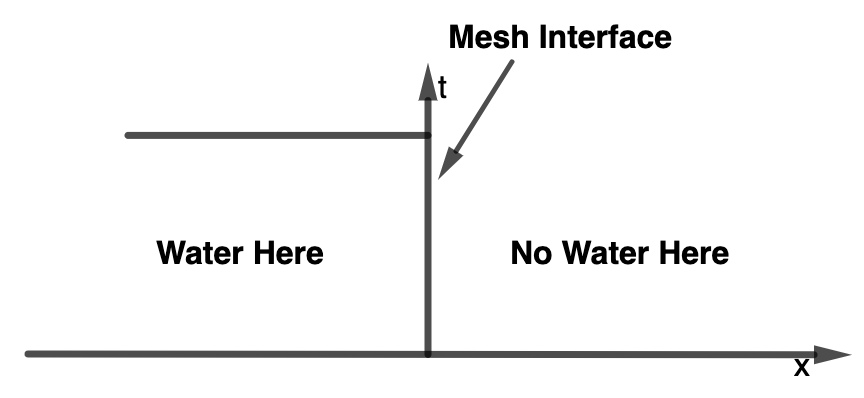
\includegraphics[width=0.5\linewidth]{images/dd1}
		\caption{ The Riemann problem with a dry bed (has no water) in one of the data state. }
		\label{fig:dry-bed}
	\end{figure}
	There are three possible cases to consider as illustrated in fig.~\ref{fig:dry-wet}. Case (a) right dry bed, the solution exhibits {\em 1-rarefaction} wave associated with the left eigenvalue $\lambda_1 = u - a$. Case (b) Left dry bed, the solution exhibits {\em 2-rarefaction} wave associated with the right eigenvalue $\lambda_2 = u + a$. Case (c) dry bed doesn't exit at $t=0$, but is created in the interaction between the two left and right wet bed regions if $S_{*L} \le S_{*R}$ where $a = \sqrt{gh}$ \cite{toro2001shock}.
	

Many more other techniques to manage dry/wet interfaces have been proposed by various researchers in unique ways, for instance, see \citet{po:2015, po:2018, pe-bo-ma:2011, toro2001shock, chaabelasri1849simple,nikolos2009unstructured,huang2013well,fivser2016mass, bi2014finite,song2011unstructured,buttinger2019fast}.


	\subsection{Approach 1 - Liu}
					Similarly, \citet{li-ta-wa-ca-ba-ch-li:2021} used the same approach to process dry and wet/dry front cells to predict flood elevation by modifying the dry cell's center elevation to correspond to the averaged peak of the two surrounding intercell heights. However, in \cite{ge:2008}, George used an approximate Riemann solver for the shallow water equations (SWE) to decompose an augmented solution vector into four propagating waves. This maintained excellent features in the approximate solution, such as preserving depth non-negativity, shockwave solutions capturing, e.t.c., making the solver appropriate for modeling SWE when steady states and dry cells exist.


	\subsection{Relaxation method (Pelanti)}

	\subsection{Toro's approach}

	\subsection{Bunya's approach}

				\citet{bu-ku-we-da:2009} modeled wetting and drying for the piecewise linear Runge-Kutta discontinuous Galerkin approximation to the SWE, which achieved positivity of the mean water depth within each finite element by using a fixed mesh approach. Additionally, instabilities caused due to excessive drying were handled by particular computation of the numerical flux.   
		The wetting and drying can also be handled by the linear piecewise  Runge-Kutta discontinuous Galerkin approximation (RKDG)  to SWE solutions; this method is based on the thin water layer approach to optimize both computational cost and accuracy on fixed meshes. The water depth of each dry or partially wet element is tracked and controlled by updating water surface elevations at every end of each Runge-Kutta time step. This maintains the depth positivity of the water column through redistributing mass within each element, which brings about a stable solution over the entire domain for the SWE \cite{bu-ku-we-da:2009}. In addition, local mass is conserved since the sum of mass inside an element remains constant. The update is independent of the neighboring elements states because it highly depends on the element's velocity and surface elevation. The technique's special treatment of numerical fluxes enables the water mass positivity in each element \cite{bu-ku-we-da:2009,kubatko2007semi}. According to \citet{bokhove2005flooding,bu-ku-we-da:2009}, the locality minimizes the communication between subdomains which improves parallel efficiency. However, RKDG and MUSCL approaches all have  the same way as the FVM of extending to get higher order. 


	\subsection{Augmented Riemann solver (George)}

	\subsubsection{WPA for the Shallow Water Equations}
	The combination of equations in system \eqref{p2}, forms a system of one-dimensional SWEs given by equation \eqref{p3}
	
	\begin{eqnarray}
		\begin{bmatrix} h \\ hu \end{bmatrix}_t + \begin{bmatrix} uh \\ hu^{2} + \frac{1}{2} gh^{2} \end{bmatrix}_x  = 0 
		\label{p3}
	\end{eqnarray}
	Equation \eqref{p3} can be written as a quasi-linear system as shown in equation \eqref{p4}:
	
	\begin{equation}
		\begin{bmatrix} h \\ hu \end{bmatrix}_t + 
		\begin{bmatrix} 0 &  1 \\ -u^{2} + gh & 2u \end{bmatrix} 
		\begin{bmatrix} h \\ hu \end{bmatrix}_x =  
		\begin{bmatrix} 0 \\ 0 \end{bmatrix}
		\label{p4}
	\end{equation}
	where the flux Jacobian matrix $f'(q)$ is given by 
	\begin{equation}
		f'(q) = \begin{bmatrix} 0 &  1 \\ -u^{2} + gh & 2u \end{bmatrix} 
		\label{ep}
	\end{equation}
	The non linear problem (equation \eqref{fvm0}), can be replaced by a linearized problem defined locally at each cell interface \cite{le-ge-be:2011},
	\begin{equation}
		\hat{q}_t + \hat{A}_{i-\frac{1}{2}}  \hat{q}_x  = 0
		\label{n2}
	\end{equation}
	where $2 \times 2$ matrix $\hat{A}_{i-\frac{1}{2}} $ (equation \eqref{n3}) is selected to be an approximation of $f^{\prime}(q)$ that is valid in the neighbourhood of the intial data $Q_{i-1}$ and $Q_{i}$.
	\begin{equation}
		\hat{A}_{i-\frac{1}{2}} =  \begin{bmatrix} 0 &  1 \\ -\hat{u}^{2} + g\bar{h} & 2\hat{u} \end{bmatrix} 
		\label{n3}
	\end{equation}
	where $\bar{h} = \frac{1}{2}(h_{i-1} + h_{i})$ is the average between end points $h_{i-1}$ and $h_{i}$, $g$ is the acceleration due to gravity, and $\hat{u} = (\sqrt{h_{i-1} }u_{i-1} + \sqrt{h_i}u_i)/(\sqrt{h_{i-1}} + \sqrt{h_i})$ is the Roe average. Since $\hat{A}_{i-\frac{1}{2}} $ is a real diagonalizable Jacobian matrix evaluated at $\hat{q} = (\bar{h},\bar{h}\hat{u})$, then its eigenvalues ($\hat{\lambda}$) and eigenvectors ($\hat{r}$) are given by equations  \eqref{eg} and \eqref{vec} respectively \cite{leveque2001class}.
	\begin{equation}
		\hat{\lambda}^1 = \hat{u} - \hat{c}, \qquad 	\hat{\lambda}^2 = \hat{u} + \hat{c}
		\label{eg}
	\end{equation}
	
	\begin{equation}
		\hat{r}^1 =  \begin{bmatrix} 1 \\ 	\hat{\lambda}^1 \end{bmatrix}, \qquad 	\hat{r}^2 =  
		\begin{bmatrix} 1 \\ 	\hat{\lambda}^2 \end{bmatrix}
		\label{vec}
	\end{equation}
	where $\hat{c} = \sqrt{gh}$, the approximate Riemann solver is used to decompose the vector  $ \delta \equiv Q_{i} - Q_{i-1}$ into two waves: $\alpha_{i-\frac{1}{2}}^{1} \hat{r}^1$ and $\alpha_{i-\frac{1}{2}}^{1} \hat{r}^2$ as 
	\begin{equation}
		Q_{i} - Q_{i-1} = \alpha_{i-\frac{1}{2}}^{1} \hat{r}^1 + \alpha_{i-\frac{1}{2}}^{1} \hat{r}^2 \equiv \mathcal{W}_{i-\frac{1}{2}}^{1} + \mathcal{W}_{i-\frac{1}{2}}^{2}
	\end{equation}
	where the coefficients $\alpha_{i-\frac{1}{2}}^{1}$ are given by:
	\begin{eqnarray}
		\alpha_{i-\frac{1}{2}}^{1} &=& \frac{(\hat{u} + \hat{c})\delta^{1} - \delta^2}{2\hat{c}}\\
		\alpha_{i-\frac{1}{2}}^{2} &=& \frac{-(\hat{u} - \hat{c})\delta^{1} + \delta^2}{2\hat{c}}
	\end{eqnarray}

	Here, we describe the approach taken by \citet{ge:2008}.  \citet{leveque2001class} proposed that equation \eqref{p3} can be decomposed into equation \eqref{p5}:

	\begin{equation}
		\begin{bmatrix} 
			H_{i} - H_{i-1}\\ 	HU_{i} - HU_{i-1} \\  \varphi(Q_{i}) - \varphi(Q_{i-1}) 
		\end{bmatrix} = \sum_{p=1}^{3} \alpha_{i-\frac{1}{2}}^{p} w_{i-\frac{1}{2}}^{p}
		\label{p5}
	\end{equation}
	where the momentum flux $\varphi(q) = (hu^{2} + \frac{1}{2} gh^{2})$, $Q_{i} = (H_{i},HU_{i})^{T}$ represents the numerical solution of $q = (h,hu)^{T}$ in $C_{i}$, and $w_{i-\frac{1}{2}}^{p} \in \mathbb{R}^{3}$ ,$\forall ~ p \in [1,3] $ with $p$ a set of chosen independent vectors. \\
	
	The decomposition of the solutions $Q_{i} - Q_{i-1} $  and  $f(Q_{i}) - f(Q_{i-1})$ $ \in  \mathbb{R}^{2}$ are represented by the first two and last two components of the three components of the decomposition \eqref{p5} respectively.  Conservation is maintained by modifying fluctuations using the last two of the three components  in equation \eqref{p5} \cite{ba-le-mi-ro:2003}. Then  consider $z_{i-\frac{1}{2}}^{p} \in \mathbb{R}^{2}$ for each $p \in [1,3]$ to be flux waves defined by:
	
	\begin{equation}
		z_{i-\frac{1}{2}}^{p} = [\mathbf{0}_{2\times1} \quad \mathbf{I}_{2\times2}] \alpha_{i-\frac{1}{2}}^{p} w_{i-\frac{1}{2}}^{p}
	\end{equation}
	where $\mathbf{0}_{2\times1}$ is a two by one zeros matrix, $\mathbf{I}_{2\times2}$ is a two by two identity. Then updated fluctuations become:
	\begin{eqnarray}
		\mathcal{A^{+}}\Delta Q_{i-\frac{1}{2}}^{n} = \sum_{\{ p:s_{i-\frac{1}{2}}^{p}>0\}}  z_{i-\frac{1}{2}}^{p}
		\label{p7}\\
		\mathcal{A^{-}}\Delta Q_{i+\frac{1}{2}}^{n} = \sum_{\{ p:s_{i+\frac{1}{2}}^{p}<0\}} z_{i+\frac{1}{2}}^{p}
		\label{p8}
	\end{eqnarray}
	Equations \ref{p7} and \ref{p8} are determined by decomposing flux in a similar way as in the f-wave approach in \citet{ba-le-mi-ro:2003} and \citet{george2006finite}, however in  \citet{ge:2008}  its decomposed into three waves ($w^{p}_{i-\frac{1}{2}} ~\in ~\mathbb{R}^{3}$)  with three associated wave speeds ($s^{p}_{i-\frac{1}{2}} ~\text{for}~ p =1,2,3$)  rather than two  allowing a more accurate approximation to the Riemann problem with a large rarefaction and a natural entropy fix for transonic rarefactions. The first and third eigen pairs $\{w^{1,3}_{i-\frac{1}{2}},s^{1,3}_{i-\frac{1}{2}}\}  $    are related to the eigen pairs of \eqref{ep}, even though in  \citet{be-ge-le-ma:2011}, its the first and second pairs that relate to the original fields of SWE. \\
	

	\section{ Future research directions}
	
	
	
	
	%\nocite{*}
	
	\bibliographystyle{abbrvnat}
	%\bibliographystyle{plain}
	\bibliography{geoclaw,literature}
	
\end{document}

